\documentclass[10pt,twocolumn]{article}
\usepackage[margin=0.72in]{geometry}
\usepackage{amsmath,amssymb}
\usepackage{graphicx}
\usepackage{booktabs}
\usepackage{caption}
\usepackage[hidelinks]{hyperref}
\usepackage{microtype}
\graphicspath{{figures/}}
\captionsetup{font=small,labelfont=bf}
\setlength{\parskip}{1.5pt}
\newcommand{\sharpe}{\ensuremath{\mathrm{SR}}}

\title{\vspace{-2.5em}\bfseries Do Candlestick-Image CNNs Predict Crypto Returns?\\
\normalsize A Pre-Registered, Survivorship-Corrected Replication (Extended Abstract)}
\author{Author Name\quad\texttt{aps9412@gmail.com}}
\date{\today}

\begin{document}
\twocolumn[
\begin{@twocolumnfalse}
\maketitle
\begin{abstract}
\noindent We test whether the candlestick-image CNN of Jiang, Kelly \& Xiu (2023, \emph{JF})---which
predicts equity returns from pictures of price charts---transfers to cryptocurrency. To avoid
data-mining, the entire design (a four-cell image$\times$horizon grid, $365$-day annualization, and a
cost grid) was \emph{pre-registered}, and every Sharpe is reported with its multiple-testing
correction, transaction cost, benchmark comparison, and a \emph{direct} survivorship measurement that
crypto uniquely permits (exchanges retain delisted coins). On a point-in-time top-100 Binance universe
(out-of-sample 2021--2026), two of four configurations survive Bonferroni correction ($\sharpe=1.47$,
$1.09$); their edge is not a survivorship artifact (measured bias $\approx 0$), beats buy-and-hold,
momentum, reversal, a trend factor, and a Kalman estimator, and is factor-orthogonal. The deep
architecture is decisive at the $20$-day horizon (a linear model on the same pixels scores $0.21$ vs
the CNN's $1.09$) but only incremental at $5$ days. The binding constraint is economic: under a
conservative endogenous spread estimate (Corwin--Schultz), only the low-turnover configuration remains
non-negative. The honest verdict is a \emph{statistically genuine but economically fragile} signal.
\vspace{1em}
\end{abstract}
\end{@twocolumnfalse}
]

\section{Motivation}
A CNN trained on \emph{images} of OHLC candlestick charts---no returns, no fundamentals, only the
picture---predicts the sign of future US-equity returns \cite{jkx}. We ask whether this transfers to
cryptocurrency: a $24/7$ market with no fundamentals, extreme volatility, and a short,
survivorship-hostile history. If a chart-image CNN carries a real edge it should appear in a different
market; if it was an equities artifact, crypto should expose it. The hazard is that a high-capacity
model searched over many settings always yields \emph{some} good Sharpe, so our contribution is as much
methodological as empirical: pre-registration, multiple-testing correction, benchmark anchoring, and a
direct measurement of survivorship bias.

\section{Data and method}
We use daily Binance klines (2018--2026), which---unlike equity vendors---\emph{retain delisted
coins}: of the $618$ assets that pass through our universe, $436$ ($71\%$) are delisted yet present with
full history. Two locked choices were amended before estimation and disclosed: the universe is ranked
by trailing dollar volume (no free point-in-time market cap exists), and pre-2020 USD prices are
cross-rated through BTC (concentrated in training, $\approx\!0$ in the test window). We split symbols at
trading gaps and at $>\!5\times$ jumps spanning a halt to remove ticker-reuse and redenomination
artifacts (e.g.\ LUNA's spurious $+177{,}399\times$ ``return''), keeping genuine crashes. Every feature
passes a leakage corruption test.

The image encoding and network are Jiang--Kelly--Xiu's \texttt{TrendCNN} reproduced verbatim; the
network sees only the image. Labels are $\mathbf{1}\{r_{t\to t+H}>0\}$ with an exactly-$H$-day holding
period; we train through 2020 (five-member ensemble) and evaluate 2021--2026. Portfolios are
equal-weight top-minus-bottom decile books rebalanced every $H$ days on the continuous grid, annualized
at $365/H$. Inference uses Bonferroni and Benjamini--Hochberg across the four-cell family and a
stationary block bootstrap.

\section{Results}
\paragraph{Corrected grid (Table~\ref{tab:main}).} Two of four configurations survive Bonferroni:
the ``fast'' I5/R5 ($\sharpe=1.47$, $p=0.002$) and ``slow'' I20/R20 ($\sharpe=1.09$, $p=0.044$); the
off-diagonal cells fail. The Deflated Sharpe Ratio \cite{dsr} (correcting for trials, skew, kurtosis,
length) is $0.91$ and $0.96$.

\paragraph{Survivorship, measured not assumed.} Re-introducing the bias (restricting to survivors)
changes I5/R5 by $-0.001$ and \emph{lowers} I20/R20 by $0.21$: the edge is not manufactured by dropping
dead coins---if anything a survivor-selected universe understates it. This is the measurement equity
data usually cannot make.

\paragraph{Benchmarks.} On identical rows, both winners beat every benchmark---buy-and-hold BTC
($0.51$), equal-weight top-100, momentum, one- and one-month reversal, the Han--Zhou--Zhu trend factor,
and a Kalman trend/vol estimator ($0.71$, a genuine opponent). Return-stream correlations with reversal
($|\rho|\le0.38$) and with BTC ($|\rho|\le0.07$) are low: the signal is neither repackaged reversal nor
hidden market beta.

\paragraph{Is the deep net needed?} A logistic regression and gradient-boosted trees on the \emph{same}
pixels reveal a horizon split: at $5$ days a linear model already reaches $1.03$ (CNN $1.47$), but at
$20$ days it collapses to $0.21$ while the CNN holds $1.09$. Deep learning earns its keep for the
slower, nonlinear pattern.

\paragraph{The economic constraint (Fig.~\ref{fig:costs}).} Replacing flat costs with a per-coin
effective spread estimated from daily highs and lows \cite{cs}---a deliberately conservative
upper bound (it assigns even BTC $71$ bps vs a true few)---destroys the high-turnover I5/R5 ($\sharpe
\to -1.48$) and leaves only I20/R20 non-negative ($\to +0.05$). The edge is short-concentrated;
removing the alt-coin short (long-only, or hedged with a liquid BTC short) cuts the Sharpe to
$0.31$/$0.06$. The signal is real; its net-of-friction profitability is marginal.

\begin{table}[t]
\centering
\caption{Pre-registered grid, out-of-sample. Two cells survive Bonferroni; both have near-zero
survivorship bias. ``CS-net'' is net of the conservative Corwin--Schultz spread.}
\label{tab:main}
\small
\begin{tabular}{lcccc}
\toprule
Config & \sharpe & Bonf.\ $p$ & Surv.\ bias & CS-net \\
\midrule
\textbf{I5/R5}   & \textbf{1.47} & 0.002 & $-0.00$ & $-1.48$ \\
\textbf{I20/R20} & \textbf{1.09} & 0.044 & $-0.21$ & $+0.05$ \\
I20/R5           & 0.78 & 0.266 & $-0.01$ & --- \\
I5/R20           & 0.11 & 1.000 & $+0.32$ & --- \\
\bottomrule
\end{tabular}
\end{table}

\begin{figure}[t]
\centering
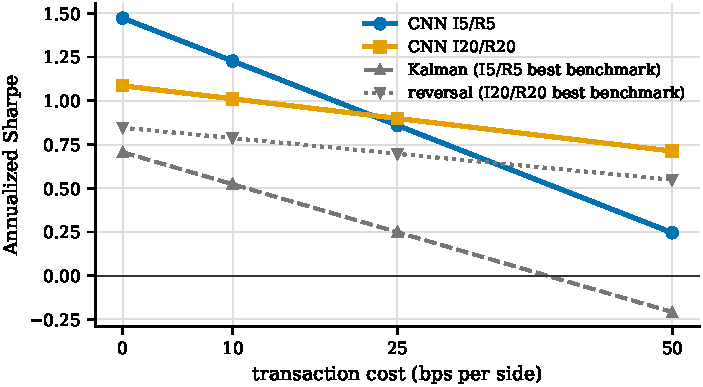
\includegraphics[width=\linewidth]{fig_costs.pdf}
\caption{Cost sensitivity. The fast cell (I5/R5) starts higher but decays steeply with turnover; the
slow cell (I20/R20) is nearly cost-flat and dominates beyond $\sim\!25$ bps.}
\label{fig:costs}
\end{figure}

\section{Verdict}
Under a pre-registered, survivorship-corrected, benchmark-anchored protocol, the candlestick-CNN
produces a \emph{statistically genuine} cross-sectional signal in two of four crypto configurations: it
survives Bonferroni and deflated-Sharpe correction, is not a survivorship artifact, beats every
benchmark, and---at the $20$-day horizon---requires the deep architecture. Its limitation is
\emph{economic}: short-concentrated and, under conservative spreads, only marginally net-positive in its
low-turnover form. The result is real enough to reject ``chart images carry nothing,'' but not yet shown
to be net-profitable after the frictions of shorting illiquid coins. Natural next steps are a second
exchange and walk-forward retraining. All code and a forward paper-trading harness are released.

\begin{thebibliography}{9}
\small
\bibitem{jkx} J.~Jiang, B.~Kelly, D.~Xiu. (Re-)Imag(in)ing price trends. \emph{J.\ Finance}
78(6):3193--3249, 2023.
\bibitem{cs} S.~Corwin, P.~Schultz. A simple way to estimate bid-ask spreads from daily high and low
prices. \emph{J.\ Finance} 67(2):719--760, 2012.
\bibitem{dsr} D.~Bailey, M.~L\'opez de Prado. The deflated Sharpe ratio. \emph{J.\ Portfolio Mgmt.}
40(5):94--107, 2014.
\end{thebibliography}

\end{document}
